\documentclass[12pt,a4paper,fontset=mac]{ctexart}
\usepackage[margin=2.2cm]{geometry}
\usepackage{graphicx,booktabs,amsmath,float,xcolor,listings}
\usepackage{longtable,array,caption}
\usepackage[hidelinks]{hyperref}
\setCJKmonofont{PingFang SC}
\graphicspath{{images/}}
\setlength{\emergencystretch}{2em}
\setlength{\parskip}{0.25em}
\renewcommand{\arraystretch}{1.18}
\captionsetup{font=small,labelfont=bf}
\lstset{language=Python,basicstyle=\ttfamily\footnotesize,
 keywordstyle=\color{blue!70!black},commentstyle=\color{green!40!black},
 stringstyle=\color{orange!60!black},showstringspaces=false,breaklines=true,
 breakatwhitespace=false,columns=fullflexible,keepspaces=true,frame=single,
 tabsize=4,numbers=left,numberstyle=\tiny\color{gray},numbersep=6pt,
 xleftmargin=1em,aboveskip=0.8em,belowskip=0.8em}

\newcommand{\reporttitle}{实验二：存储层次设计空间探索}
\newcommand{\subtask}{L1D 容量、相联度与替换策略、块大小、MSHR 及 L2 权衡}
\newcommand{\authname}{姓名}
\newcommand{\authid}{学号}
\newcommand{\class}{班级}

\title{\reporttitle\\[0.4em]\large\subtask}
\author{\small\authname：\underline{李祥熙}\quad
\authid：\underline{2234412799}\quad\class：\underline{计算机2301}}
\date{2026年11月20日}

\begin{document}
\maketitle

\begin{abstract}
本实验基于 gem5 25.0.0.1（RISC-V SE 模式，O3 乱序处理器），围绕 int8 量化神经网络推理负载 \texttt{qnn}（工作集约 100.7 KiB，随机种子 2799）及无空间局部性对照负载 \texttt{pchase}，系统探索 L1D 容量、相联度与替换策略、Cache 块大小、MSHR 深度与 L2 容量对性能的影响。实验表明：在容量—延迟权衡模型下，L1D 在 8--64 KiB 区间因无法容纳工作集且命中延迟随容量递增而单调变慢，至 128 KiB 处发生拐点（周期数降至 $905\,805$，较 32 KiB 基线加速 $1.217\times$）；64 KiB 下 LRU 在 2/4/8 路组相联中发生循环扫描颠簸，反而不如直接映射与随机替换；块大小从 16 B 增至 256 B 时 \texttt{l1d\_mshr\_mpki} 按 2 倍精确减半（与理论预测误差仅约 0.5\%），而 16 B 的性能崩塌并非 MSHR 不足，而是取指缓冲受限于 16 B 导致 I-Cache 停顿占总周期的 66.6\%；将 MSHR 从 1 增至 2 会使 \texttt{l1d\_miss\_rate} 从 0.78\% 跃升至 12.30\% 而 \texttt{l1d\_mshr\_mpki} 保持 2.211 不变，说明失效率是微体系结构产物而非程序固有属性；L2 在 128 KiB 时已完全容纳工作集，继续增大仅增加访问延迟。最终给出面向有限硅片面积的综合配置提案（\texttt{l1d-size=128kB}、\texttt{l1d-assoc=2}、\texttt{cacheline=128}、\texttt{l2-size=256kB}），实测在 \texttt{qnn} 上获得 $1.217\times$ 加速，在 \texttt{pchase} 上获得 $1.178\times$ 加速，并揭示了参数间交互作用与延迟/替换策略模型的边界。
\end{abstract}

\clearpage
\tableofcontents
\newpage

\section{实验目的}
\begin{itemize}
  \item 在固定硅片面积预算约束下，通过受控设计空间探索（DSE）分析 L1D 容量、相联度与替换策略、块大小、MSHR 数量及 L2 容量对执行周期的影响。
  \item 理解命中延迟随容量增长的物理权衡（AMAT 模型），辨析仿真器缺失关键物理模型时产生的假结论。
  \item 通过 3C 模型与替换策略实验，理解循环顺序扫描下 LRU 颠簸的机理以及相联度与替换策略的耦合关系。
  \item 掌握“先定量预测、后实测验证”与“提出假设、构造反例、定位真因”的体系结构实验方法，区分真实下级流量（\texttt{l1d\_mshr\_mpki}）与被次级失效放大的 \texttt{l1d\_miss\_rate}。
  \item 提出有数据支撑的综合存储层次配置提案，并通过多参数实测与跨负载验证评估参数交互及结论稳健性。
\end{itemize}

\section{实验环境与方法}
\subsection{软硬件环境与基线配置}
实验主机为 Apple M4（10 核、16 GiB 内存），操作系统为 macOS 27.0.1，仿真器为 gem5 25.0.0.1（RISC-V SE 模式），Python 3.11.15。所有实验均使用学号后四位 \texttt{2799} 作为随机种子，依据实验一确定的环境噪声地板（约 0.01\%），小于 0.1\% 的差异一律视为无显著差异。表~\ref{tab:baseline} 给出默认基线参数（命令行中的 \texttt{kB} 按 gem5 实际解释为二进制单位 KiB）。

\begin{table}[H]\centering\small
\caption{实验二默认基线配置（相对基线均以此为参照）}\label{tab:baseline}
\begin{tabular}{ll}\toprule
参数 & 默认取值 \\\midrule
CPU 模型 & O3 乱序处理器（2 GHz，8 宽取指/发射/提交） \\
L1D 容量与相联度 & 32 KiB，2 路组相联，LRU 替换 \\
L1D MSHR 数量 & 4 \\
Cache 块大小 & 64 B（同时作用于 L1I / L1D / L2） \\
L2 容量与相联度 & 256 KiB，8 路组相联 \\
延迟缩放模型 & \texttt{--auto-latency on}（以 32 KiB / 3 周期为基准，每翻一番 +1 周期） \\
核心负载 & \texttt{qnn}（\texttt{8 2799}，ROI 指令数 $5\,800\,766$） \\
对照负载 & \texttt{pchase}（\texttt{256 200000 2799}，256 KiB 随机指针环，20 万跳） \\
\bottomrule\end{tabular}
\end{table}

\subsection{核心工作集分析与核心指标}
\texttt{qnn} 实现 $784\to128\to10$ 的 int8 量化两层感知机推理，其静态数据工作集尺寸为：权重矩阵 \texttt{w1[128][784]} 占 $100\,352$ B（约 98 KiB），\texttt{w2[10][128]} 占 $1\,280$ B，偏置 \texttt{b1[128]} 占 512 B，输入缓冲 \texttt{xbuf[784]} 占 784 B，其余变量约 208 B，合计约 \textbf{100.7 KiB}（$103\,117$ B）。

在非阻塞 Cache 中，失效次数满足：
\begin{equation}
\mathrm{overallMisses} = \mathrm{overallMshrHits} + \mathrm{overallMshrMisses}, \qquad
\mathrm{MLP} = \frac{\mathrm{overallMisses}}{\mathrm{overallMshrMisses}}.
\end{equation}
由于乱序核在数据返回前会持续向同一缺失块发射访存请求并合并为 MSHR hit，实验统一采用 \texttt{l1d\_mshr\_mpki}（每千条指令真正下发到 L2 的失效请求数）衡量真实访存压力，以 ROI 周期数（\texttt{cycles}）作为最终性能指标。

\section{实验过程、结果与机制分析}

\subsection{任务 1：L1D 容量与延迟权衡（寻找拐点）}
分别在 \texttt{--auto-latency on} 与 \texttt{--auto-latency off} 下扫描 L1D 容量（8 KiB 至 256 KiB）。关键执行命令如下：
\begin{lstlisting}[language=bash,caption={任务 1 容量扫描命令}]
python3 framework/sweep.py --name task1_size \
  --bench qnn --bench-args "8 2799" --base "--cpu o3" \
  --vary l1d-size=8kB,16kB,32kB,64kB,128kB,256kB --jobs 6

python3 framework/sweep.py --name task1_size_nolat \
  --bench qnn --bench-args "8 2799" --base "--cpu o3 --auto-latency off" \
  --vary l1d-size=8kB,16kB,32kB,64kB,128kB,256kB --jobs 6
\end{lstlisting}

表~\ref{tab:task1} 给出两组扫描的实测数据，图~\ref{fig:capacity} 在对数横轴上对比了两条周期曲线。

\begin{table}[H]\centering\footnotesize\setlength{\tabcolsep}{4.5pt}
\caption{任务 1：L1D 容量扫描结果（\texttt{auto-latency on} 与 \texttt{off} 对照）}\label{tab:task1}
\begin{tabular}{lrrrrrrr}\toprule
L1D 容量 & 周期数（on） & IPC（on） & \texttt{miss\_rate} & \texttt{l1d\_mpki} & \texttt{mshr\_mpki} & 周期数（off） & IPC（off） \\\midrule
8 KiB   & 1\,050\,028 & 5.524 & 11.57\% & 32.726 & 2.212 & 1\,102\,100 & 5.263 \\
16 KiB  & 1\,076\,306 & 5.390 & 12.31\% & 34.829 & 2.212 & 1\,102\,100 & 5.263 \\
32 KiB  & 1\,102\,090 & 5.263 & 12.32\% & 34.873 & 2.211 & 1\,102\,090 & 5.263 \\
64 KiB  & 1\,142\,571 & 5.077 & 12.32\% & 34.852 & 2.210 & 1\,102\,059 & 5.264 \\
128 KiB & \textbf{905\,805} & \textbf{6.404} & 0.01\%  & 0.039  & 0.002 & \textbf{887\,006} & \textbf{6.540} \\
256 KiB & 1\,009\,789 & 5.745 & 0.01\%  & 0.041  & 0.002 & 887\,006    & 6.540 \\
\bottomrule\end{tabular}
\end{table}

\begin{figure}[H]\centering
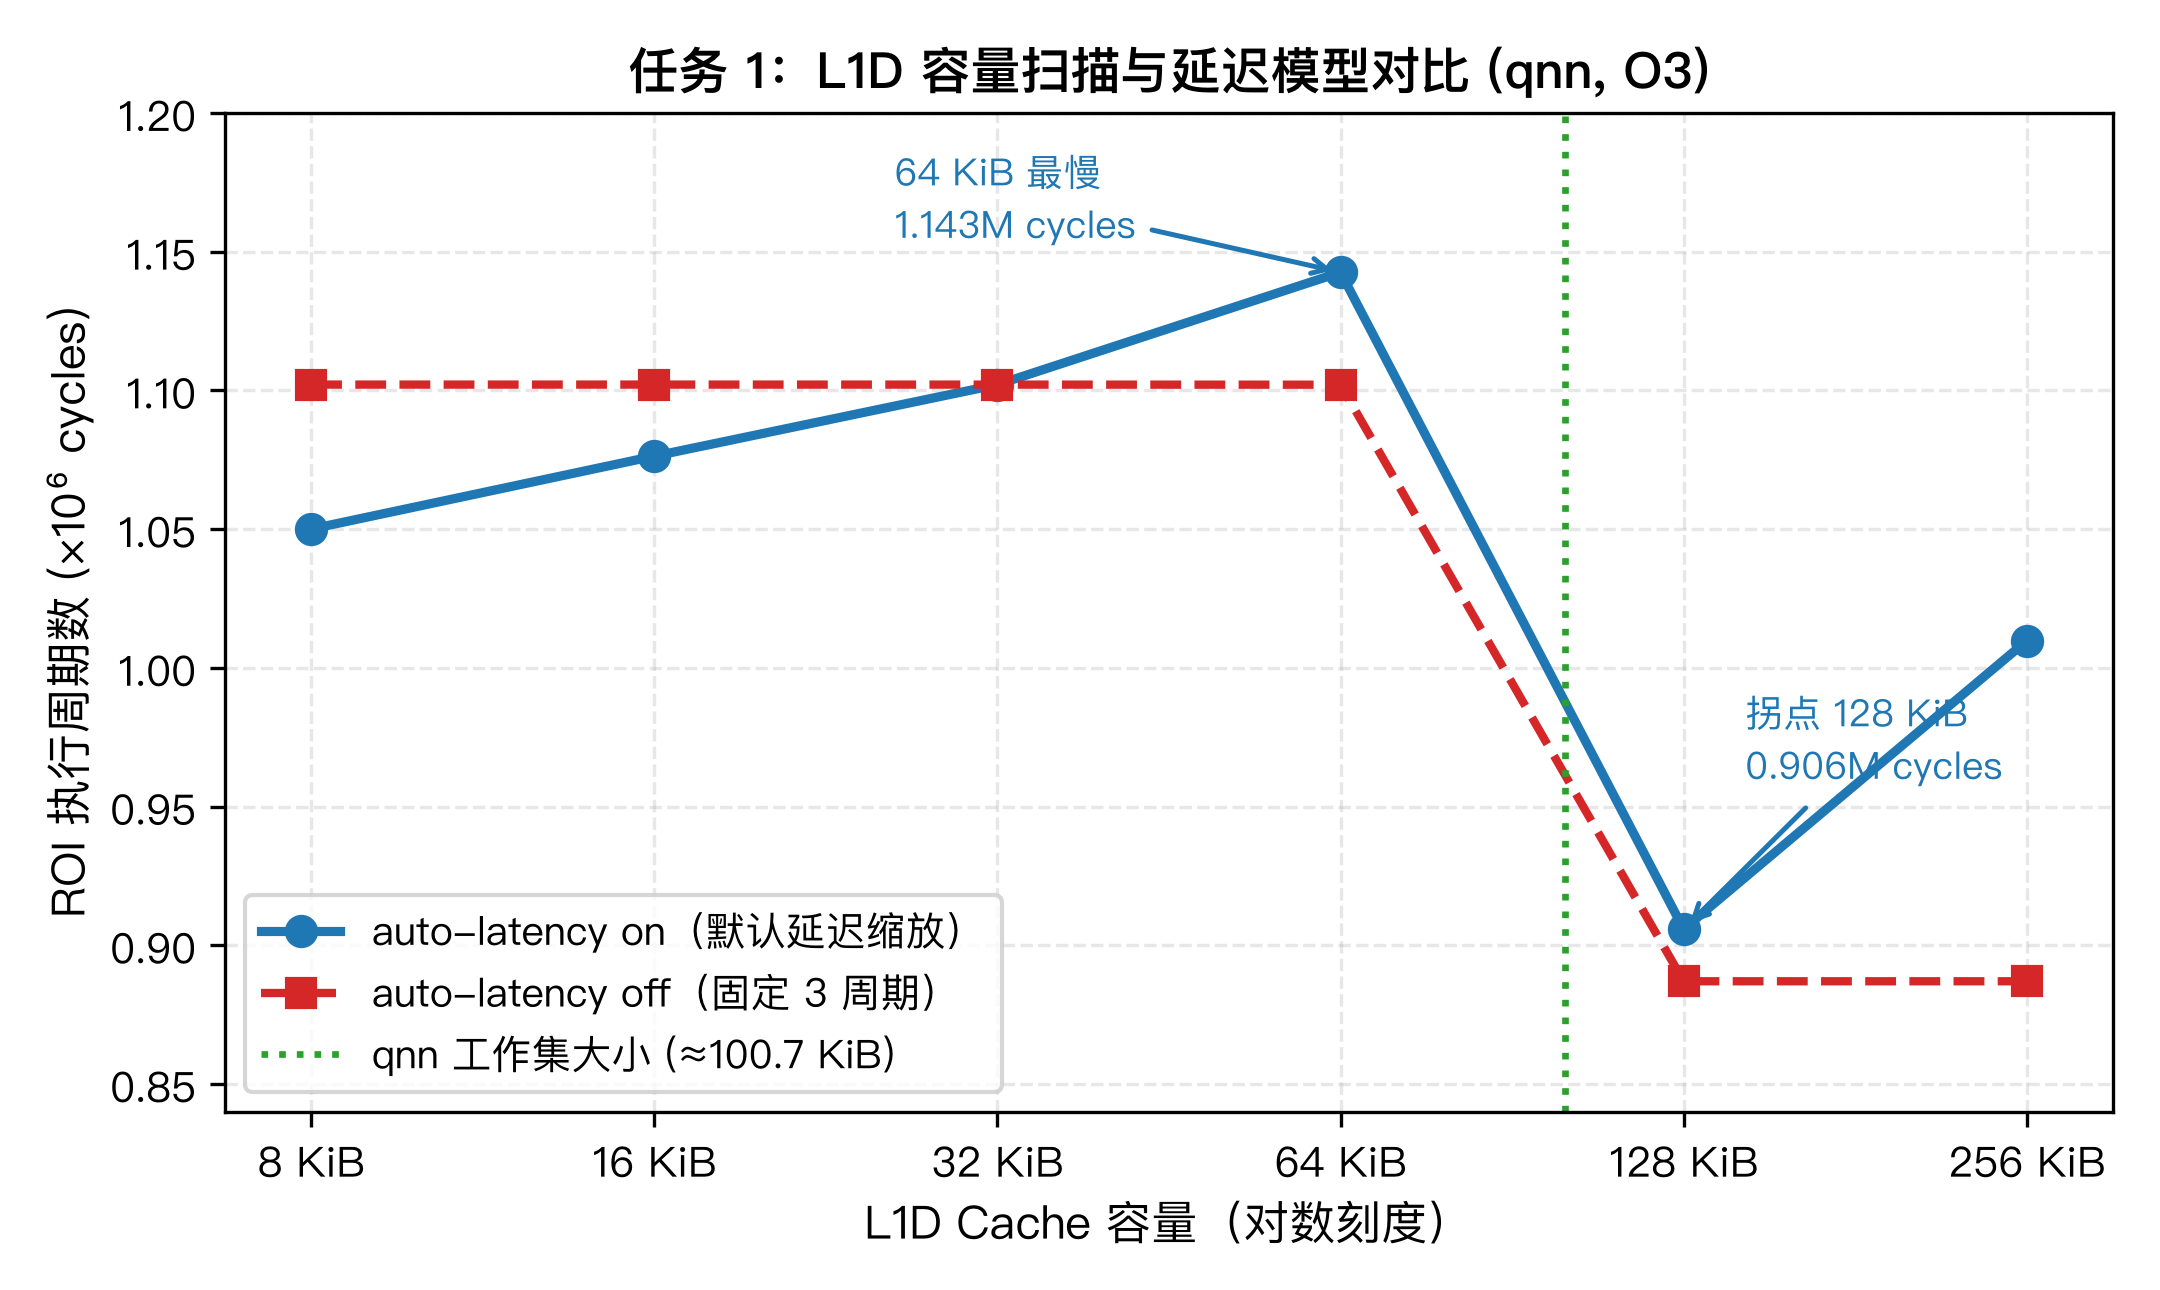
\includegraphics[width=0.86\textwidth]{fig1_capacity.png}
\caption{任务 1：L1D 容量扫描周期曲线（\texttt{auto-latency on} 与 \texttt{off} 对比）}
\label{fig:capacity}
\end{figure}

从表~\ref{tab:task1} 与图~\ref{fig:capacity} 可直接回答任务 1 的全部问题：
\begin{enumerate}
  \item \textbf{最优容量与加速比：}周期数最少的是 \textbf{128 KiB}（$905\,805$ 周期），较 32 KiB 基线（$1\,102\,090$ 周期）减少 17.81\% 的周期，加速比为 \textbf{1.217$\times$}。
  \item \textbf{8 KiB $\to$ 64 KiB 反而变慢的原因：}该区间内 \texttt{l1d\_mshr\_mpki} 几乎完全不变（$2.212 \to 2.210$），说明在容量超过 100.7 KiB 工作集之前，增大容量并未带来任何失效收益；而 \texttt{scaled\_latency()} 使命中延迟每翻一番增加 1 周期（$1 \to 2 \to 3 \to 4$ 周期）。收益为零而命中延迟代价持续上升，导致 64 KiB 成为全程最慢点（$1\,142\,571$ 周期）。
  \item \textbf{128 KiB 处的突变：}\texttt{qnn} 工作集约 100.7 KiB，当 L1D 达到 128 KiB 时整个工作集（尤其是 98 KiB 的 \texttt{w1}）首次完整驻留 L1D，容量失效瞬间消失，\texttt{l1d\_mshr\_mpki} 从 2.210 骤降至 0.002，周期数出现陡降拐点。
  \item \textbf{256 KiB 重新变慢：}128 KiB 已基本消除所有失效（\texttt{l1d\_mshr\_mpki} 维持 0.002），扩至 256 KiB 没有任何失效收益，却多付出了 1 个周期的命中延迟（$5 \to 6$ 周期），导致周期数回升至 $1\,009\,789$（变慢 11.48\%）。
  \item \textbf{关闭延迟模型后的曲线与假结论：}关闭 \texttt{--auto-latency} 后，曲线呈单调阶梯下降（8--64 KiB 平坦于 $1.102\times10^6$，128--256 KiB 平坦于 $8.870\times10^5$）。若仅看此曲线，会得出“容量越大越好、256 KiB 至少不差于 128 KiB”的错误结论。
  \item \textbf{模型真实性判断：}\texttt{auto-latency on} 更接近真实芯片，因为 SRAM 容量翻倍必然导致字线/位线变长、寄生电容增大、译码器层数与 Tag 扇出增加，命中延迟客观上升。
  \item \textbf{方法学推广：}仿真器未建模的物理约束（如面积、功耗、线延迟）都会在结果中以“免费午餐”的形式出现，诱导设计者将对应参数推向极端，因此任何实验结论都必须在所建模型的边界内解释。
\end{enumerate}

\subsection{任务 2：相联度与替换策略的反直觉交互（核心任务）}
首先在 LRU 替换下扫描容量（32/64/128 KiB）与相联度（1/2/4/8 路），随后在 64 KiB 下对比 LRU 与 Random 替换策略。表~\ref{tab:task2a} 与表~\ref{tab:task2b} 给出实测结果，图~\ref{fig:assoc_repl} 展示 64 KiB 下相联度与替换策略的交互效应。

\begin{table}[H]\centering\small
\caption{任务 2(a)：不同容量与相联度下的 \texttt{l1d\_mshr\_mpki}（LRU 替换）}\label{tab:task2a}
\begin{tabular}{lrrrr}\toprule
L1D 容量 & 1 路（直接映射） & 2 路 & 4 路 & 8 路 \\\midrule
32 KiB \texttt{mshr\_mpki}  & 2.272 & 2.211 & 2.210 & 2.210 \\
\textbf{64 KiB \texttt{mshr\_mpki}} & \textbf{1.632} & \textbf{2.210} & \textbf{2.210} & \textbf{2.210} \\
128 KiB \texttt{mshr\_mpki} & 0.002 & 0.002 & 0.002 & 0.002 \\
\bottomrule\end{tabular}
\end{table}

\begin{table}[H]\centering\small
\caption{任务 2(b)：64 KiB L1D 下 LRU 与 Random 替换策略对比}\label{tab:task2b}
\begin{tabular}{crrrr}\toprule
相联度 & LRU \texttt{mshr\_mpki} & LRU 周期数 & Random \texttt{mshr\_mpki} & Random 周期数 \\\midrule
1 路 & 1.632 & 1\,075\,795 & 1.632 & 1\,075\,795 \\
2 路 & 2.210 & 1\,142\,571 & 1.584 & 1\,078\,119 \\
4 路 & 2.210 & 1\,142\,571 & 1.496 & 1\,070\,414 \\
8 路 & 2.210 & 1\,142\,571 & 1.457 & 1\,067\,003 \\
\bottomrule\end{tabular}
\end{table}

\begin{figure}[H]\centering
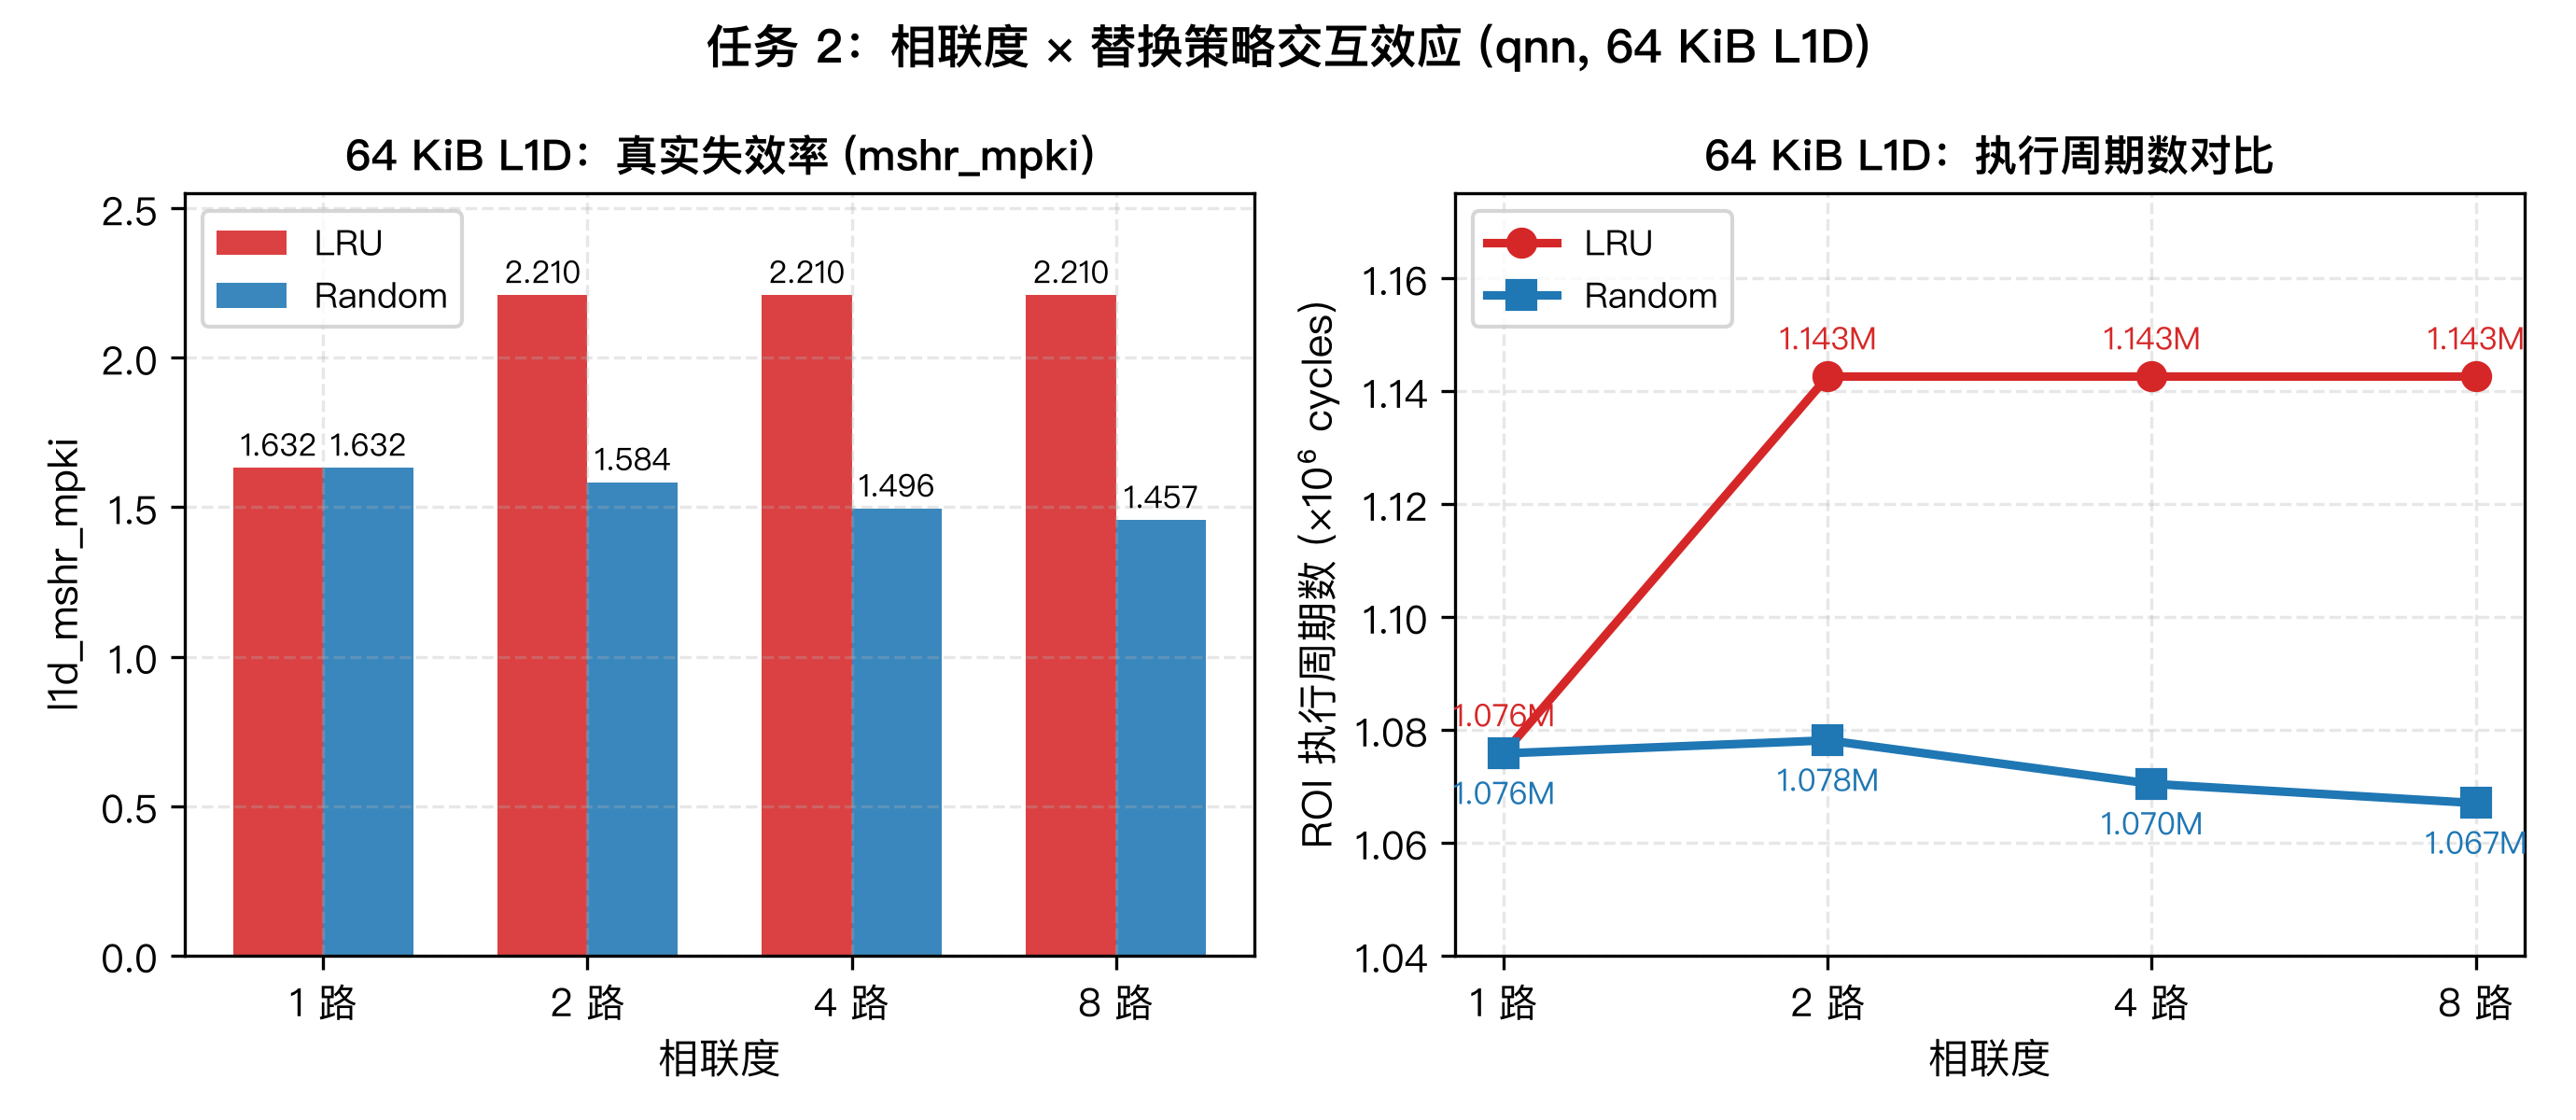
\includegraphics[width=0.95\textwidth]{fig2_assoc_repl.png}
\caption{任务 2：64 KiB L1D 下相联度与替换策略（LRU vs. Random）的对比}
\label{fig:assoc_repl}
\end{figure}

机制分析如下：
\begin{enumerate}
  \item \textbf{反教科书现象（问题 1）：}在 64 KiB 下，\textbf{1 路（直接映射）的失效数（1.632）显著少于 2/4/8 路 LRU（2.210）}，失效减少了 26.2\%，周期数快了 5.84\%（$1\,075\,795$ vs. $1\,142\,571$）。这与“提高相联度总能减少失效”的直觉相反。
  \item \textbf{3C 模型的隐含前提（问题 2）：}标准 3C 模型中“提高相联度不会增加失效”的结论隐含了\textbf{替换策略是最优（Belady MIN）或至少不发生病态颠簸}的前提，实际上将失效分类当成了与替换策略无关的性质。但在固定容量下，提高相联度会减少组数（$\text{组数} = C / (B \times A)$），从而缩短组索引覆盖的地址跨度，当替换策略为 LRU 时反而可能放大颠簸。
  \item \textbf{1 路自检（问题 3）：}表~\ref{tab:task2b} 中 1 路时 LRU 与 Random 结果完全一致（\texttt{mshr\_mpki} 均为 1.632，周期数均为 $1\,075\,795$）。因为直接映射每组只有 1 个槽位，替换对象唯一确定，替换策略不发挥任何作用，结果必须完全相同。
  \item \textbf{单调性对比（问题 4）：}在 Random 策略下，随着相联度从 1 路升至 8 路，\texttt{mshr\_mpki} 严格单调下降（$1.632 \to 1.584 \to 1.496 \to 1.457$），周期数也降至 $1\,067\,003$；而在 LRU 下，从 1 路升至 2 路后失效反而暴涨至 2.210 并完全停滞。
  \item \textbf{LRU 落败的机理（问题 5）：}\texttt{qnn} 内层循环 \texttt{dot\_i8(w1[j], xbuf, 784)} 每次顺序扫描 784 B，每个样本将 98 KiB 的 \texttt{w1} 从头到尾线性遍历一遍，随后在下一个样本重新回到开头。
  \begin{itemize}
    \item 在 64 KiB、1 路直接映射下，地址跨度为 64 KiB，98 KiB 阵列回卷后仅有前/后各 34 KiB 映射到冲突组，中间约 \textbf{30 KiB 的组只对应唯一地址}，因此这约 $30/98 \approx 30.6\%$ 的数据常驻 Cache 并持续命中（实测减少 26.2\% 失效，扣除 \texttt{xbuf} 等辅数组后高度吻合）。
    \item 在 2/4/8 路组相联下，组索引跨度缩短为 32/16/8 KiB，98 KiB 的 \texttt{w1} 均匀覆盖所有组，使每组映射的块数（如 2 路约 3.06 块/组）全部超过相联度。当扫描至数组末尾准备回到开头时，LRU 保留的是刚刚用过的数组末尾 64 KiB，而马上要访问的开头部分已被全部逐出，导致每一轮重用率跌至 0\%（完全颠簸）。Random 替换则以概率随机保留部分旧块，打破了“必定逐出下一次最先使用块”的最坏周期性。
  \end{itemize}
  \item \textbf{设计结论与真实处理器实践（问题 6）：}对于\textbf{工作集略大于 Cache 容量的顺序循环扫描模式}，不应采用纯 LRU。真实处理器中，Intel L1 通常采用 \textbf{Tree-PLRU}（伪 LRU），ARM Cortex 系列 L1 常采用 \textbf{Pseudo-Random} 或 PLRU，而现代处理器的 L2/L3 则普遍引入抗扫描/抗颠簸策略（如 RRIP/DRRIP/QLRU）。L1 不用标准 LRU 的核心原因有二：一是硬件代价高（8 路精确 LRU 需要维护 $8!=40\,320$ 种排序状态，更新逻辑拖慢 L1 命中关键路径并增加功耗）；二是纯 LRU 在循环扫描下极易发生 0\% 命中率的灾难性颠簸。
\end{enumerate}

\subsection{任务 3：Cache 块大小——三股力量的拔河（核心任务）}
\subsubsection{先预测、后测量（任务 3a）}
依据工作集 $100.7\ \text{KiB} = 103\,117\ \text{B}$、8 个样本及约 $5.8\times10^6$ 条 ROI 指令，在运行前通过脚本 \texttt{tmp.py} 计算理论预测值：
\begin{lstlisting}[language=Python,caption={任务 3(a) 事前定量预测脚本（tmp.py）}]
WORKING_SIZE = 103_117  # 100.7 KiB in bytes
SAMPLE = 8
INSTRUCTION = 5_800_000
cacheline = [16, 32, 64, 128, 256]

misses_per_sample = [WORKING_SIZE / c for c in cacheline]
mshr_mpki = [m * SAMPLE * 1000 / INSTRUCTION for m in misses_per_sample]
# 预测结果: [8.889, 4.445, 2.222, 1.111, 0.556]
\end{lstlisting}

表~\ref{tab:task3a} 将预测值与 \texttt{task3a\_line.csv} 实测值对照，图~\ref{fig:cacheline} 给出可视化结果。

\begin{table}[H]\centering\footnotesize\setlength{\tabcolsep}{4.5pt}
\caption{任务 3(a)/(b)：块大小预测与实测对比（\texttt{qnn}，32 KiB L1D）}\label{tab:task3a}
\begin{tabular}{crrrrrrr}\toprule
块大小 & 预测每样本失效 & 预测 \texttt{mshr\_mpki} & 实测 \texttt{mshr\_mpki} & 相对误差 & 实测周期数 & IPC & \texttt{l1d\_mlp} \\\midrule
16 B  & 6\,444.8 & 8.889 & 8.841 & +0.54\% & 4\,985\,034 & 1.164 & 2.996  \\
32 B  & 3\,222.4 & 4.445 & 4.421 & +0.54\% & 1\,294\,809 & 4.480 & 15.729 \\
64 B  & 1\,611.2 & 2.222 & 2.211 & +0.50\% & 1\,102\,090 & 5.263 & 15.769 \\
128 B & 805.6    & 1.111 & 1.106 & +0.45\% & 1\,006\,720 & 5.762 & 15.768 \\
256 B & 402.8    & 0.556 & 0.554 & +0.36\% & 959\,226    & 6.047 & 15.732 \\
\bottomrule\end{tabular}
\end{table}

\begin{figure}[H]\centering
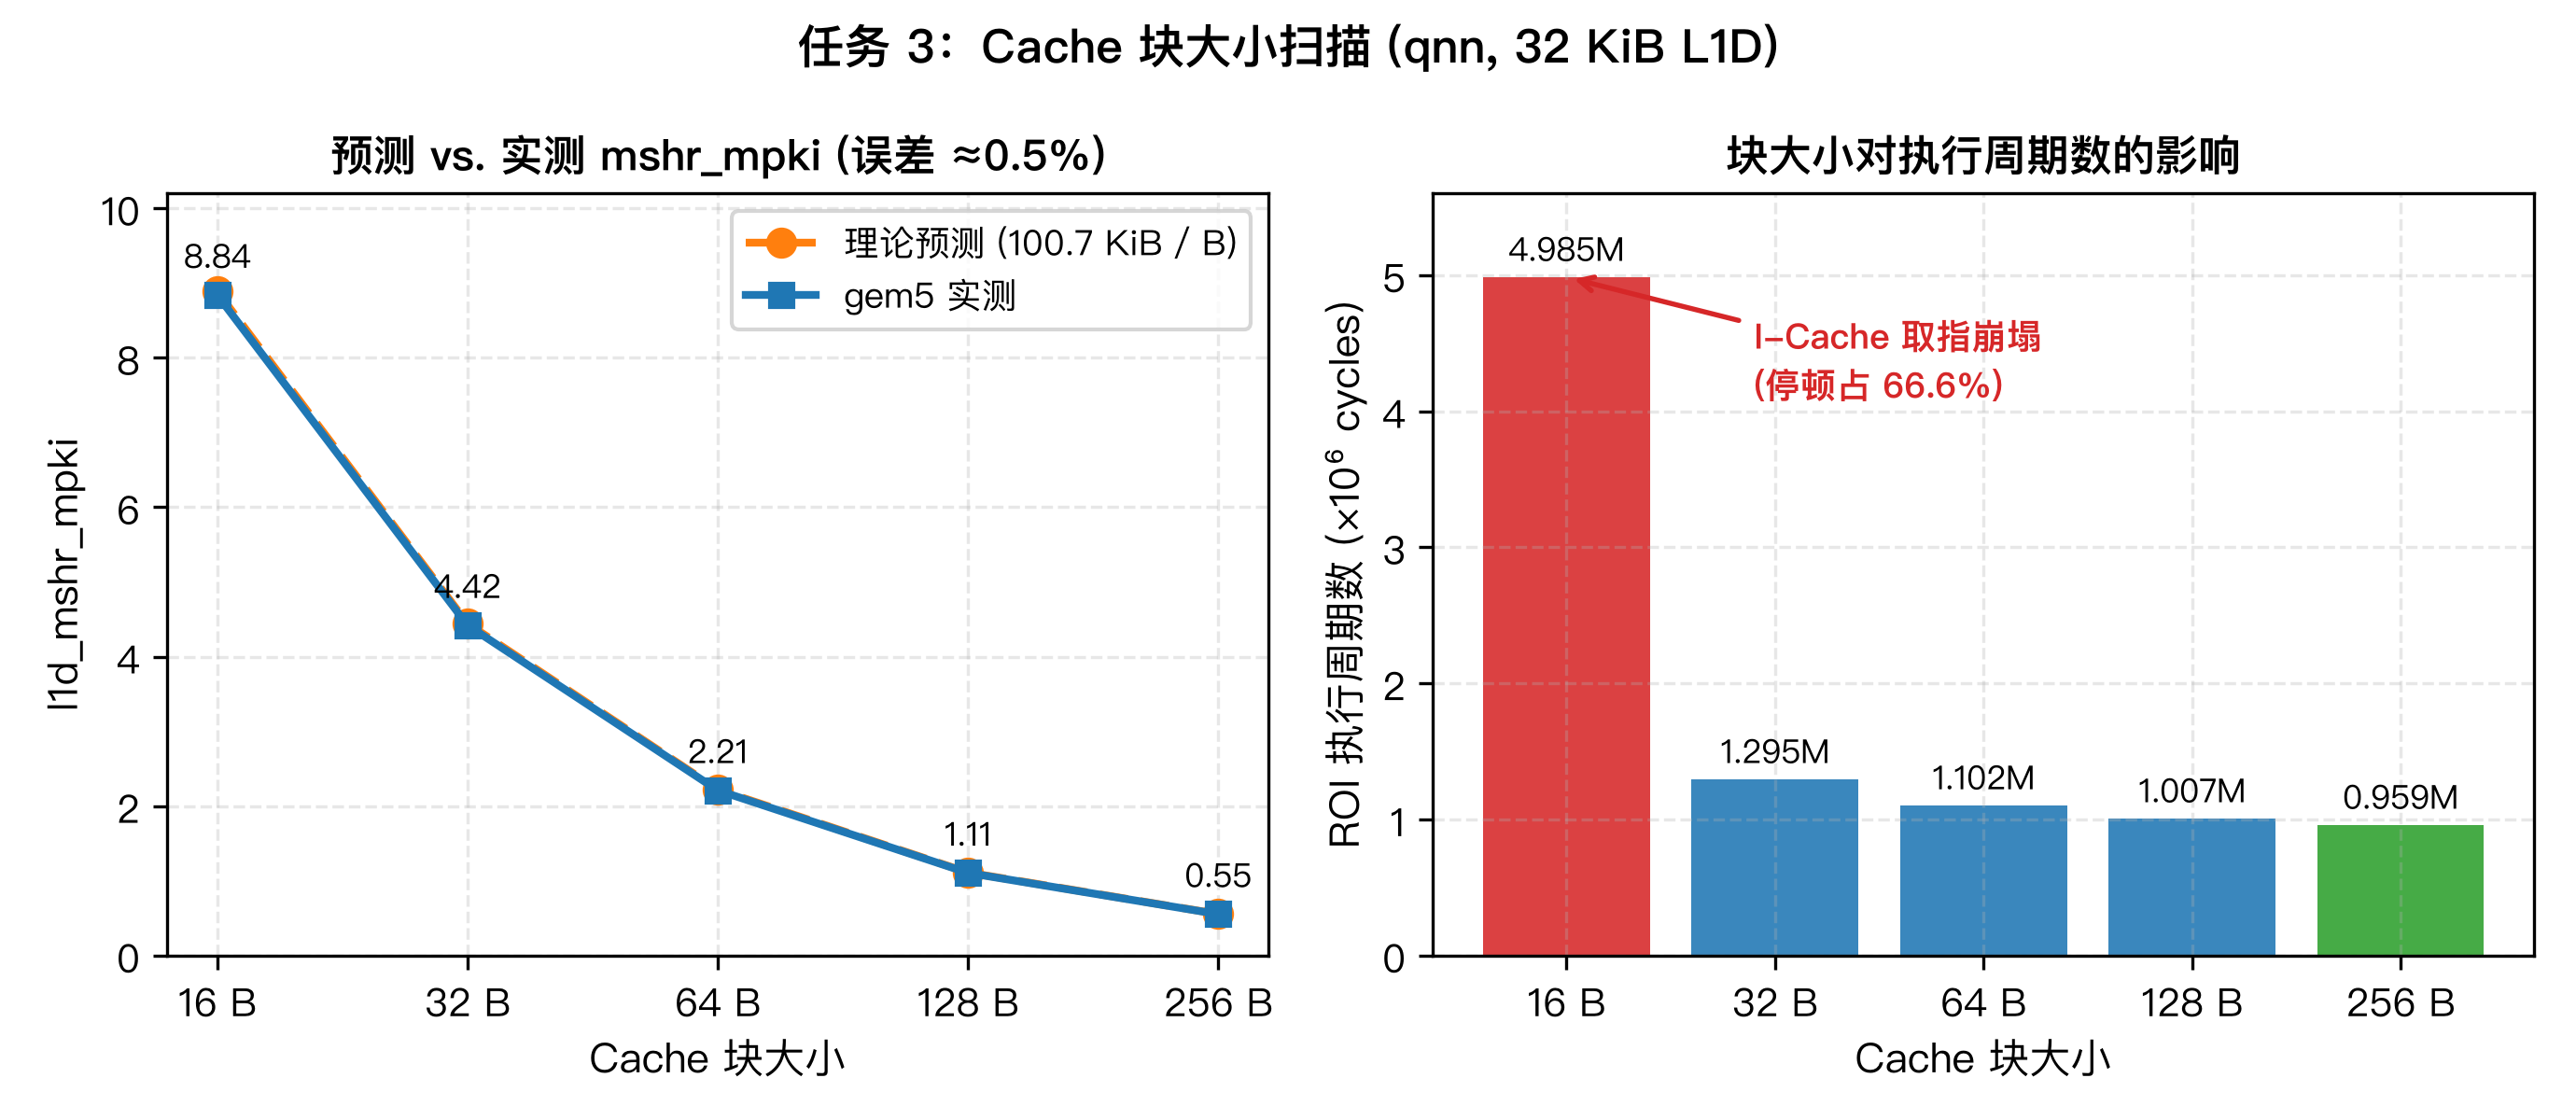
\includegraphics[width=0.95\textwidth]{fig3_cacheline.png}
\caption{任务 3：Cache 块大小对 \texttt{l1d\_mshr\_mpki}（预测 vs. 实测）及执行周期的影响}
\label{fig:cacheline}
\end{figure}

\begin{itemize}
  \item \textbf{预测精度与规律（问题 1--2）：}五个块大小的预测误差全部在 \textbf{0.36\%--0.54\%} 之间，高度吻合。块大小每翻一倍，\texttt{l1d\_mshr\_mpki} 精确减半（$8.841 \to 4.421 \to 2.211 \to 1.106 \to 0.554$）。原因在于 \texttt{dot\_i8} 对 \texttt{w1} 进行 100\% 连续顺序访问，每个样本搬运的总字节数（约 100.7 KiB）恒定不变，单块容量翻倍自然使总搬运块数减半。
  \item \textbf{周期数为何不成比例下降（问题 3）：}从 16 B 到 256 B，失效数降了 16 倍，周期数仅降了 5.20 倍（若看正常的 32 B $\to$ 256 B 区间，失效数降 8 倍，周期数仅降 1.35 倍）。这受限于 \textbf{Amdahl 定律}（即使 L1D 零失效，计算与命中基线仍需约 $9\times10^5$ 周期）以及乱序核高内存级并行（\texttt{l1d\_mlp} $\approx 15.7$）对 L2 访存延迟的有效掩盖。
\end{itemize}

\subsubsection{16 B 性能崩塌的假设检验与真因定位（任务 3b 问题 4--5）}
16 B 块的周期数骤增至 $4\,985\,034$（比 32 B 慢 3.85 倍），且 \texttt{l1d\_mlp} 暴跌至 2.996。首先检验“MSHR 不够用”的假设：将 \texttt{l1d-mshrs} 扩增至 16 和 64 并检查 \texttt{dcache.blockedCycles::no\_mshrs}，结果见表~\ref{tab:task3mshr} 与嵌入的 \texttt{grep} 统计。

\begin{table}[H]\centering\small
\caption{任务 3(b)：扩大 MSHR 数量对 16 B / 32 B / 64 B 的影响}\label{tab:task3mshr}
\begin{tabular}{ccrrrr}\toprule
块大小 & \texttt{l1d-mshrs} & 周期数 & IPC & \texttt{l1d\_mshr\_mpki} & \texttt{l1d\_mlp} \\\midrule
16 B & 4 / 16 / 64 & 4\,985\,034 / 4\,985\,061 / 4\,985\,089 & 1.164 & 8.841 & 2.996 \\
32 B & 4 / 16 / 64 & 1\,294\,809 / 1\,294\,535 / 1\,294\,535 & 4.480 & 4.421 & 15.729 \\
64 B & 4 / 16 / 64 & 1\,102\,090 / 1\,102\,090 / 1\,102\,090 & 5.263 & 2.211 & 15.769 \\
\bottomrule\end{tabular}
\end{table}

\begin{lstlisting}[language={},caption={16 B 与 64 B 在 ROI 段（第 2 次 dump）的阻塞与取指统计}]
# dcache.blockedCycles::no_mshrs (ROI 段，所有配置均为 0)
p000_cacheline-16_l1d-mshrs-4  (ROI):  0
p001_cacheline-16_l1d-mshrs-16 (ROI):  0
p002_cacheline-16_l1d-mshrs-64 (ROI):  0

# 16 B 取指侧统计 (ROI 段)
system.cpu.numCycles                          4985034
system.cpu.fetch.cacheLines                   1661088
system.cpu.fetchStats0.icacheStallCycles      3321370   # 占总周期 66.63%

# 64 B 取指侧统计 (ROI 段)
system.cpu.numCycles                          1102090
system.cpu.fetch.cacheLines                      4546
system.cpu.fetchStats0.icacheStallCycles         9522   # 占总周期 0.86%
\end{lstlisting}

\textbf{假设否定与真因解释：}将 MSHR 增至 64 后，16 B 的周期数纹丝不动（变化 $<0.002\%$），且 ROI 段内 \texttt{blockedCycles::no\_mshrs} 恒为 0，证明“MSHR 不足”假设不成立。真正瓶颈位于取指前端：由于 \texttt{--cacheline} 同时作用于 L1I/L1D/L2，且物理上取指单元单次最多读取一个 Cache 块（\texttt{cssys\_se.py} 中 \texttt{fetchBufferSize = min(64, cacheline)}），16 B 块使前端每次只能取出 16 字节（至多 4 条指令），导致 \texttt{fetch.cacheLines} 从 4\,546 激增 365 倍至 1\,661\,088，\texttt{icacheStallCycles} 高达 \textbf{66.63\%}（64 B 仅 0.86\%）。前端指令供给严重饥饿，使后端无法同时发射足够的 load 指令，进而导致 \texttt{l1d\_mlp} 被拖垮至 2.996。这是一个典型的“数据 Cache 参数拖垮取指单元”的跨模块耦合案例。

\subsubsection{无空间局部性负载 \texttt{pchase} 对照（任务 3b 问题 6）}
为检验块大小是否应无限增大，在 256 KiB 随机指针追逐负载 \texttt{pchase} 上对比 64 B 与 256 B，结果见表~\ref{tab:task3pchase}。

\begin{table}[H]\centering\small
\caption{任务 3(b)：\texttt{pchase}（256 KiB，20 万跳）下 64 B 与 256 B 块对比}\label{tab:task3pchase}
\begin{tabular}{ccrrrrr}\toprule
L1D 容量 & 块大小 & 周期数 & IPC & \texttt{l1d\_mshr\_mpki} & \texttt{l1d\_mlp} & \texttt{dram\_bytes} \\\midrule
32 KiB  & 64 B  & 4\,525\,841 & 0.265 & 146.933 & 1.000 & 94\,400 \\
32 KiB  & 256 B & 4\,670\,968 & 0.257 & 145.823 & 1.000 & 49\,664 \\
128 KiB & 64 B  & 3\,865\,761 & 0.310 & 86.417  & 1.000 & 70\,784 \\
128 KiB & 256 B & 3\,736\,954 & 0.321 & 84.334  & 1.000 & 32\,256 \\
\bottomrule\end{tabular}
\end{table}

\begin{itemize}
  \item \textbf{快慢结论随容量翻转：}在 \textbf{32 KiB} 下，256 B 比 64 B \textbf{慢 3.21\%}（$4.671\times10^6$ vs. $4.526\times10^6$）；而在 \textbf{128 KiB} 下，256 B 反而比 64 B \textbf{快 3.33\%}（$3.737\times10^6$ vs. $3.866\times10^6$）。
  \item \textbf{空间利用率解释：}\texttt{qnn} 对搬入的 256 B 空间利用率为 100\%；而 \texttt{pchase} 每次随机跳转仅使用单个 4 B/8 B 指针，256 B 块超过 96\% 的搬运字节是冗余的。在 32 KiB 小容量下，256 B 块将总块数压缩至仅 128 块，造成严重 Cache 污染与传输带宽浪费，微弱的失效下降（$146.93 \to 145.82$）远不足以弥补传输开销；而在 128 KiB 下，Cache 可容纳一半的 256 KiB 数组，随 256 B 块附带搬入的邻近节点有更大概率在被逐出前被后续随机跳转命中（\texttt{mshr\_mpki} 降至 84.33），从而反超 64 B。
  \item \textbf{MLP 剧烈差异的原因：}\texttt{pchase} 的 \texttt{l1d\_mlp} 恒为 \textbf{1.000}（\texttt{qnn} 约 15.7），因为指针追逐中下一次访存地址完全由当前 load 的返回值决定（真数据依赖链），乱序核无法提前计算或并行发射后续 load。
  \item \textbf{多核代价：}除浪费带宽与污染 Cache 外，大块在多核一致性系统中还会加剧\textbf{假共享（False Sharing）}——不同核心写入落在同一大块内的互不相关变量，会反复触发缓存行无效化与乒乓传输。
\end{itemize}

\subsection{任务 4：MSHR——“失效率”究竟是谁的属性}
固定 32 KiB 基线，扫描 \texttt{l1d-mshrs} $= 1, 2, 4, 8, 16$，结果见表~\ref{tab:task4}。

\begin{table}[H]\centering\small
\caption{任务 4：L1D MSHR 数量扫描结果（\texttt{qnn}，32 KiB L1D）}\label{tab:task4}
\begin{tabular}{crrrrr}\toprule
\texttt{l1d-mshrs} & 周期数 & IPC & \texttt{l1d\_miss\_rate} & \texttt{l1d\_mshr\_mpki} & \texttt{l1d\_mlp} \\\midrule
1  & 1\,115\,502 & 5.200 & \textbf{0.78\%}  & 2.211 & 1.000  \\
2  & 1\,101\,892 & 5.264 & \textbf{12.30\%} & 2.211 & 15.736 \\
4  & 1\,102\,090 & 5.263 & 12.32\% & 2.211 & 15.769 \\
8  & 1\,102\,090 & 5.263 & 12.32\% & 2.211 & 15.769 \\
16 & 1\,102\,090 & 5.263 & 12.32\% & 2.211 & 15.769 \\
\bottomrule\end{tabular}
\end{table}

\begin{enumerate}
  \item \textbf{MSHR=1 与 MSHR=2 的跳变：}\texttt{l1d\_miss\_rate} 从 \textbf{0.78\%} 暴增至 \textbf{12.30\%}（放大 \textbf{15.8 倍}），\texttt{l1d\_mlp} 从 1.000 跳至 15.736；而 \texttt{l1d\_mshr\_mpki} 始终精确维持在 \textbf{2.211}，毫无变化。原因在于 MSHR=1 时，某缓存行首次失效即占满全部 MSHR，L1D 立即阻塞并拒绝后续请求，待该行返回后同一块内其余访存全部命中；而 MSHR=2 时，仍有空闲 MSHR 维持非阻塞状态，乱序核在数据返回前持续向同一缺失行发射约 15 次访存，这些次级失效全部合并到同一 MSHR 上并计入 \texttt{overallMisses}，使表观失效率暴涨。
  \item \textbf{失效率的本质：}程序、数据与 Cache 容量全未改变，仅将队列深度从 1 改为 2 就令失效率变化近 16 倍，说明 \texttt{l1d\_miss\_rate} 是\textbf{微体系结构（乱序发射窗口与非阻塞机制）的产物}，而非程序的固有属性。
  \item \textbf{MSHR=4 $\to$ 16 无收益：}周期数恒定在 $1\,102\,090$，\texttt{l1d\_mlp} 稳定于 15.769（在 MSHR=2 时即已饱和）。因为 \texttt{qnn} 是顺序单流扫描，同时在飞的不同缺失块仅 1--2 个，大量次级失效均合并至同一 MSHR。
  \item \textbf{投资判断：}对 \texttt{qnn} 而言增加 MSHR 极不划算（2--4 个已完全足够）；只有存在大量\textbf{互不依赖的随机/多流并发缺失}（如稀疏矩阵 gather/scatter、带软件预取的图遍历、多数组 \texttt{stream}）的负载才需要更多 MSHR。
\end{enumerate}

\subsection{任务 5：L2 容量——面积应该花在哪一级}
固定 32 KiB L1D 基线，扫描 L2 容量（128 KiB 至 2 MiB），结果见表~\ref{tab:task5}。

\begin{table}[H]\centering\small
\caption{任务 5：L2 容量扫描与 DRAM 流量统计（\texttt{qnn}）}\label{tab:task5}
\begin{tabular}{lrrrrr}\toprule
L2 容量 & 周期数 & IPC & \texttt{l2\_miss\_rate} & \texttt{l2\_accesses} & \texttt{dram\_bytes} \\\midrule
128 KiB & \textbf{1\,075\,883} & \textbf{5.392} & 0.17\% & 12\,836 & 1\,600 \\
256 KiB & 1\,102\,090 & 5.263 & 0.17\% & 12\,836 & 1\,344 \\
512 KiB & 1\,127\,377 & 5.145 & 0.17\% & 12\,836 & 1\,344 \\
1 MiB   & 1\,152\,801 & 5.032 & 0.17\% & 12\,836 & 1\,344 \\
2 MiB   & 1\,178\,056 & 4.924 & 0.17\% & 12\,836 & 1\,344 \\
\bottomrule\end{tabular}
\end{table}

\begin{enumerate}
  \item \textbf{性能变化：}L2 从 128 KiB 增至 2 MiB，性能单调\textbf{变差}，周期数从 $1\,075\,883$ 升至 $1\,178\,056$，恶化幅度达 \textbf{+9.50\%}（每翻一番增加约 2.5 万周期的 L2 访问延迟）。
  \item \textbf{DRAM 流量占比：}\texttt{dram\_bytes} 绝对值仅 \textbf{1\,344--1\,600 B}（约 21--25 个 64 B 块），相对于 ROI 总访存量（约 160 万次）占比低于 \textbf{0.002\%}（\texttt{l2\_miss\_rate} 仅 0.17\%）。
  \item \textbf{架构决策：}对于 \texttt{qnn}，128 KiB L2 已完全装下 100.7 KiB 工作集，继续扩大 L2 毫无收益。架构师应将多余的 L2 面积预算优先挪给 \textbf{L1D（扩至 128 KiB）}，直接消除下发到 L2 的 12\,836 次访问。
  \item \textbf{L2 发挥价值的场景：}当负载的工作集\textbf{大于 L1D 但小于 L2}（例如 256 KiB--2 MiB 的中等规模矩阵、哈希表或中等图结构）时，L2 能拦截原本需要 100--300 周期的 DRAM 访问，此时扩大 L2 才具有决定性意义。
\end{enumerate}

\subsection{任务 6：综合配置提案与实测验证（核心交付物）}

\subsubsection{最终配置提案（不超过 400 字）}
\begin{quote}
\textbf{【配置提案】}本提案选定：\texttt{--l1d-size 128kB}、\texttt{--l1d-assoc 2}、\texttt{--cacheline 128}、\texttt{--l2-size 256kB}（LRU）。在 \texttt{qnn} 上实测 $905\,382$ 周期，较基线（$1\,102\,090$ 周期）加速 \textbf{1.217$\times$}（周期减少 17.85\%）。各维度取舍如下：（1）\textbf{L1D 选 128 KiB}：刚好跨过 \texttt{qnn} 约 100.7 KiB 工作集拐点，\texttt{mshr\_mpki} 降至 0.001；不选 8--64 KiB 是因容不下工作集导致颠簸，不选 256 KiB 是因多付命中延迟却无失效收益。（2）\textbf{相联度选 2 路}：128 KiB 下 1/2/4/8 路性能一致，不选 1 路以避免通用负载冲突失效，不选 4/8 路以节省 Tag 比较器面积与功耗。（3）\textbf{块大小选 128 B}：兼顾顺序扫描的强制失效减半与适中缓存行数，不选 16--32 B 以免取指受限，不选 256 B 以减轻随机负载污染与多核假共享。（4）\textbf{L2 选 256 KiB}：保持严格大于 L1D 并维持最低 DRAM 流量，不选 512 KiB--2 MiB 以免浪费面积并增加延迟。
\end{quote}

\subsubsection{提案实测、参数交互与跨负载验证}
表~\ref{tab:task6} 给出提案在 \texttt{qnn}（LRU 与 Random）及 \texttt{pchase}（32 KiB vs. 128 KiB）上的实测结果。

\begin{table}[H]\centering\footnotesize\setlength{\tabcolsep}{4.5pt}
\caption{任务 6：提案配置实测（\texttt{qnn}）与跨负载对照（\texttt{pchase}）}\label{tab:task6}
\begin{tabular}{llrrrrr}\toprule
负载 & 变化参数 & 周期数 & IPC & \texttt{l1d\_mshr\_mpki} & \texttt{l2\_accesses} & \texttt{dram\_bytes} \\\midrule
\texttt{qnn} & \texttt{l1d-repl=lru}    & \textbf{905\,382} & \textbf{6.407} & 0.001 & 9 & 1\,280 \\
\texttt{qnn} & \texttt{l1d-repl=random} & 906\,517 & 6.399 & 0.007 & 42 & 1\,280 \\
\midrule
\texttt{pchase} & \texttt{l1d-size=32kB}  & 4\,428\,753 & 0.271 & 146.170 & 175\,406 & 62\,976 \\
\texttt{pchase} & \texttt{l1d-size=128kB} & \textbf{3\,759\,318} & \textbf{0.319} & 84.463  & 101\,357 & 48\,000 \\
\bottomrule\end{tabular}
\end{table}

\begin{enumerate}
  \item \textbf{实测与单维外推的偏差（问题 2）：}在单维扫描中，\texttt{l1d-size=128kB} 单独带来 17.81\% 的周期缩减（降至 $905\,805$），而 \texttt{cacheline=128} 在 32 KiB 下单独带来 8.65\% 的缩减（降至 $1\,006\,720$）。若简单线性叠加，会预测组合配置可达约 $8.28\times10^5$ 周期；但实测为 \textbf{905\,382 周期}，与单改 L1D 容量（$905\,805$）相差仅 0.05\%（处于噪声地板内）。
  \item \textbf{相互影响的参数对：}\textbf{\texttt{l1d-size} 与 \texttt{cacheline}（以及 \texttt{l1d-size} 与 \texttt{l2-size}）存在强耦合}。一旦 128 KiB L1D 完整容纳 100.7 KiB 工作集，ROI 内 L2 访问次数从 12\,836 锐减至仅 \textbf{9 次}（\texttt{mshr\_mpki} $=0.001$）。既已几乎没有 L1D 失效可供块大小去减半，也几乎没有 L2 流量受 L2 延迟影响，因此单维扫描的收益不能叠加。此外，由于 \texttt{qnn} 的 ROI 从权重初始化之后开始计时，原本期待大块加速冷启动加载的效果并未落入 ROI 统计窗口内。
  \item \textbf{跨负载验证（问题 3）：}在 256 KiB 的 \texttt{pchase} 上，提案中的 128 KiB L1D 仍显著优于 32 KiB（$3\,759\,318$ vs. $4\,428\,753$，加速 \textbf{1.178$\times$}），因为 128 KiB 可缓存一半随机节点（\texttt{mshr\_mpki} 从 146.17 降至 84.46）。若换用工作集小于 32 KiB 的极小负载，或工作集远大于 128 KiB 的纯流式负载，结论则会发生翻转——此时 128 KiB 无法带来足够失效下降，反而因更高的命中延迟落败。这说明不存在脱离工作集特征的“全局最优硬件配置”。
\end{enumerate}

\section{思考题}

\subsection{思考题 1：单一指标评价设计的危险}
在任务 1 中，8 KiB L1D（$1\,050\,028$ 周期）比 64 KiB（$1\,142\,571$ 周期）快 8.10\%；若仅报告失效率（\texttt{l1d\_miss\_rate} 为 11.57\% vs. 12.32\%，或 \texttt{l1d\_mshr\_mpki} 为 2.212 vs. 2.210），甚至会误以为 64 KiB 略优或无差异。单一代理指标只反映了局部子系统的事件计数，掩盖了命中延迟增加、流水线停顿重叠及面积功耗代价，极易诱导架构师做出“局部指标变好、整机性能变差”的错误决策。

\subsection{思考题 2：延迟模型敏感性与结论稳健性}
为检验任务 1 结论对 \texttt{scaled\_latency()} 基准延迟参数的依赖，扫描 \texttt{l1-latency} $= 2, 3, 5$ 与 \texttt{l1d-size} $= 8, 32, 128, 256$ KiB，结果见表~\ref{tab:q2} 与图~\ref{fig:latsens}。

\begin{table}[H]\centering\scriptsize\setlength{\tabcolsep}{3.8pt}
\caption{思考题 2：不同基准延迟（\texttt{l1-latency}）下的容量性能与 128 KiB 领先幅度}\label{tab:q2}
\begin{tabular}{crrrrrr}\toprule
基准延迟 & 8 KiB & 32 KiB & 128 KiB & 256 KiB & 128 KiB 相对 32 KiB & 128 KiB 相对 8 KiB \\\midrule
2 周期 & 1\,047\,185 & 1\,073\,659 & \textbf{893\,929}   & 903\,508    & 1.201$\times$ (-16.74\%) & 1.171$\times$ (-14.63\%) \\
3 周期 & 1\,050\,028 & 1\,102\,090 & \textbf{905\,805}   & 1\,009\,789 & 1.217$\times$ (-17.81\%) & 1.159$\times$ (-13.74\%) \\
5 周期 & 1\,106\,874 & 1\,186\,072 & \textbf{1\,056\,771} & 1\,097\,222 & 1.122$\times$ (-10.90\%) & 1.047$\times$ (-4.53\%)  \\
\bottomrule\end{tabular}
\end{table}

\begin{figure}[H]\centering
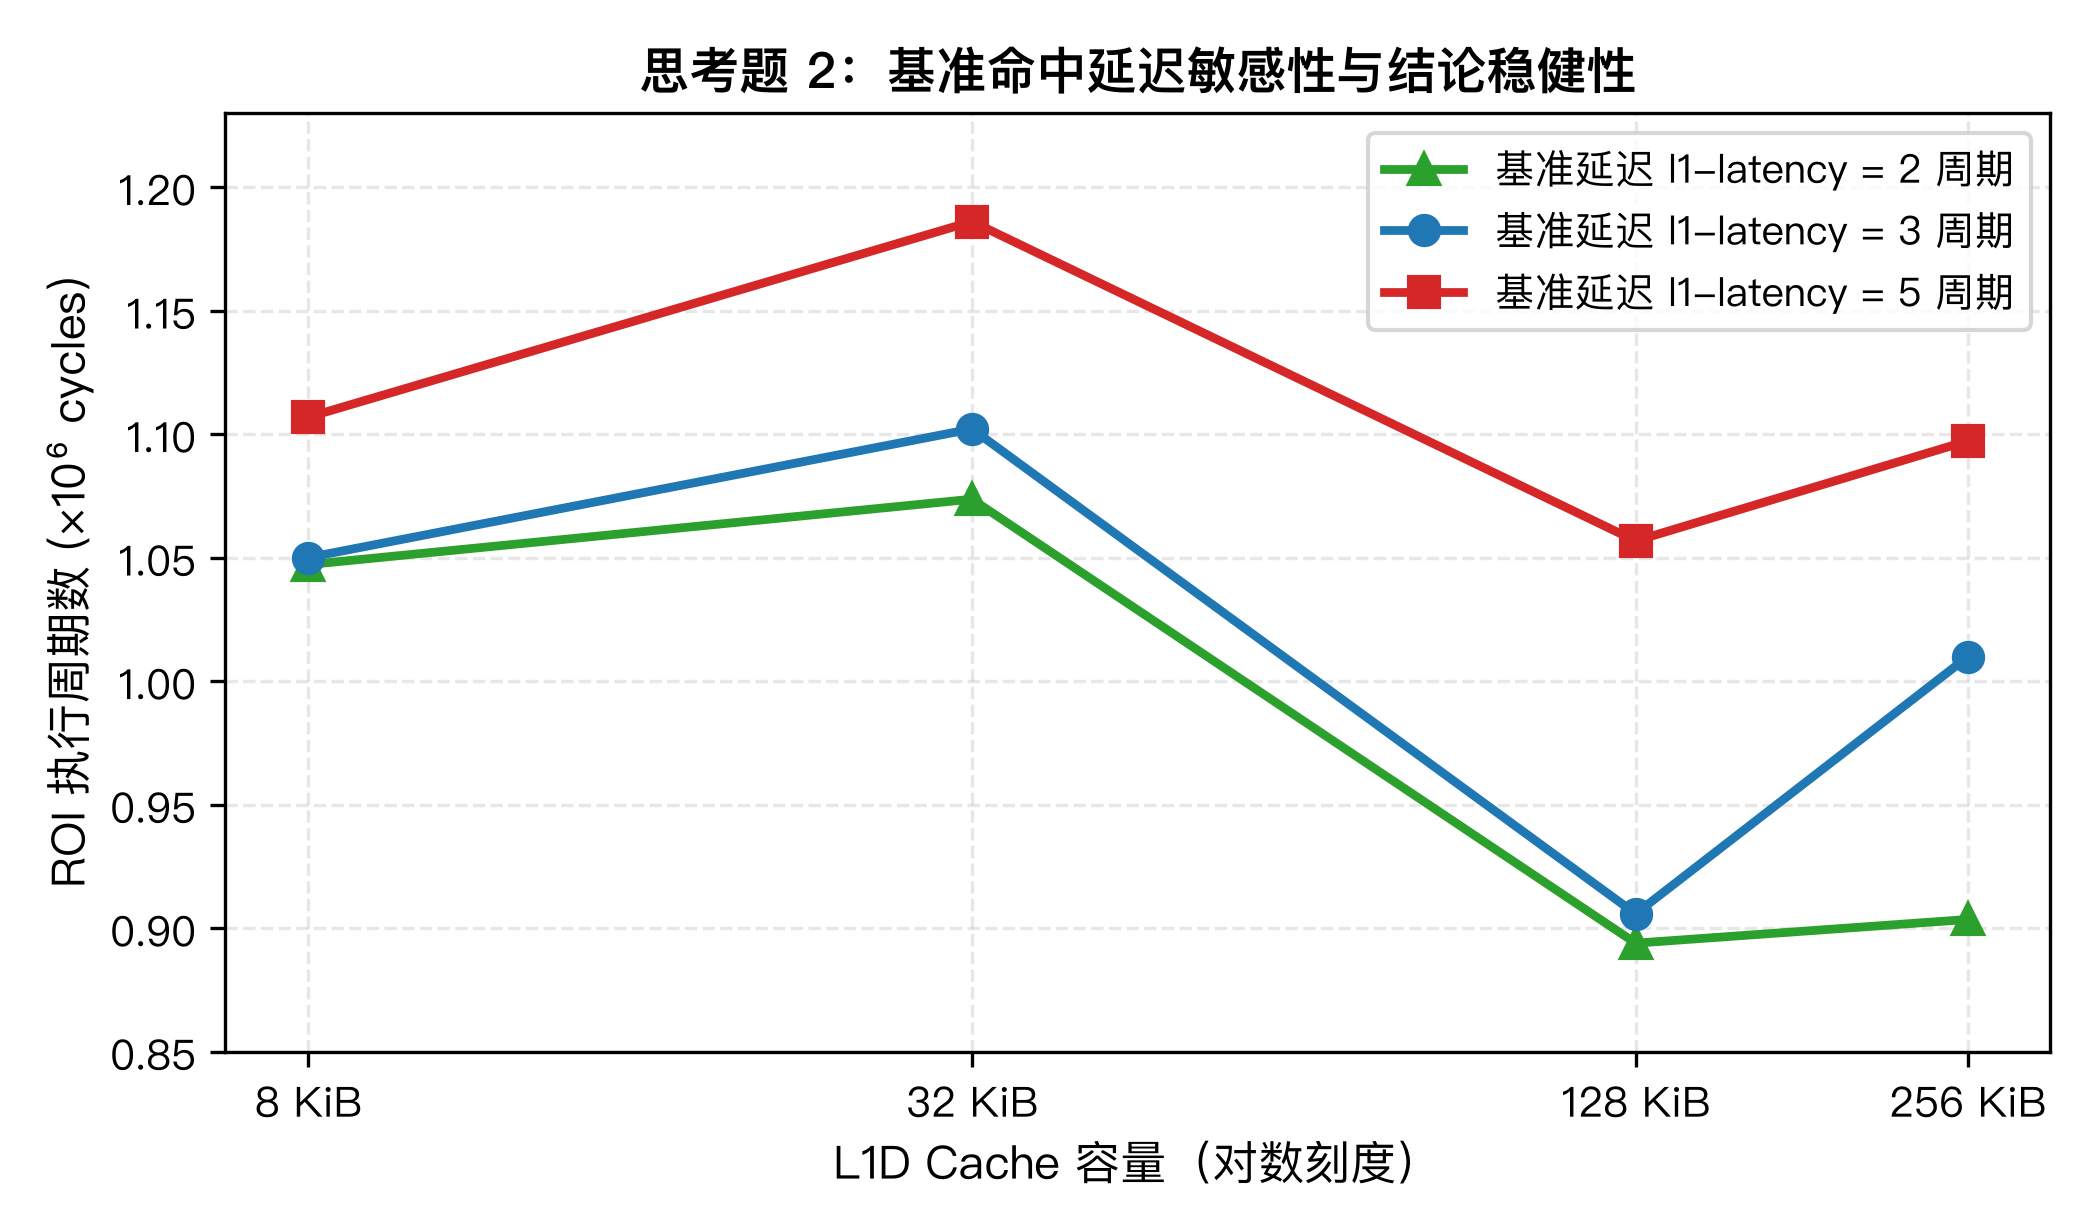
\includegraphics[width=0.82\textwidth]{fig4_latsens.png}
\caption{思考题 2：基准命中延迟（2 / 3 / 5 周期）对 L1D 容量曲线的影响}
\label{fig:latsens}
\end{figure}

\begin{itemize}
  \item \textbf{最优点的位置没有变：}无论基准延迟取 2、3 还是 5 周期，\textbf{128 KiB 始终是周期数最少的配置}。
  \item \textbf{最优点的领先幅度明显改变了：}当基准延迟升至 5 周期时，128 KiB 命中延迟达到 7 周期（8 KiB 为 3 周期），128 KiB 相对 32 KiB 的加速比从 $1.217\times$ 缩水至 $1.122\times$，相对 8 KiB 的领先幅度更是从 14.63\% 骤降至仅 \textbf{4.53\%}。定性排序在参数扰动下保持稳定、而定量收益幅度随之收窄，正是“结论稳健性”的核心含义。
\end{itemize}

\subsection{思考题 3：RRIP 抗颠簸替换策略的理论与实测对比}
\textbf{（a）RRIP 的设计目标与基本思想：}Jaleel 等人（ISCA 2010）提出的 RRIP（Re-Reference Interval Prediction）旨在解决传统 LRU 在扫描（Scan）与循环颠簸（Thrashing）负载下命中率归零的问题。它为每个缓存块维护 $M$ 位重引用间隔预测值（RRPV，0 表示近期会重用，$2^M-1$ 表示遥远重用）：\textbf{SRRIP} 将新块插入“长重用间隔”（$2^M-2$）而非 MRU，避免一次性扫描冲刷热数据；\textbf{BRRIP}（Bimodal RRIP）则以高概率（如 $1-\epsilon$）将新块插入“最远间隔”（$2^M-1$，立即成为牺牲品），仅以极小概率 $\epsilon$ 插入 $2^M-2$，从而随机钉住一部分工作集以抵抗颠簸。

\textbf{（b）64 KiB / 4 路 L1D 实测结果：}见表~\ref{tab:q3}。

\begin{table}[H]\centering\small
\caption{思考题 3：64 KiB、4 路 L1D 下六种替换策略对比（\texttt{qnn}）}\label{tab:q3}
\begin{tabular}{lrrrr}\toprule
替换策略 & 周期数 & IPC & \texttt{l1d\_miss\_rate} & \texttt{l1d\_mshr\_mpki} \\\midrule
\texttt{lru}    & 1\,142\,571 & 5.077 & 12.32\% & 2.210 \\
\texttt{random} & \textbf{1\,070\,414} & \textbf{5.419} & \textbf{8.30\%}  & \textbf{1.496} \\
\texttt{fifo}   & 1\,143\,589 & 5.072 & 12.42\% & 2.239 \\
\texttt{nru}    & 1\,142\,542 & 5.077 & 12.31\% & 2.203 \\
\texttt{rrip}   & 1\,142\,523 & 5.077 & 12.31\% & 2.205 \\
\texttt{brrip}  & 1\,142\,295 & 5.078 & 12.29\% & 2.205 \\
\bottomrule\end{tabular}
\end{table}

\textbf{（c）理论与实测不符的原因分析：}实测中 \texttt{rrip}（$1\,142\,523$）与 \texttt{brrip}（$1\,142\,295$）均未兑现抗颠簸承诺，表现与 LRU 基本一致，唯有 \texttt{random}（$1\,070\,414$）真正降低了失效。造成这一偏离的深层原因有三：
\begin{enumerate}
  \item \textbf{论文算法边界（SRRIP 不抗颠簸）：}查阅 gem5 源码 \texttt{ReplacementPolicies.py} 可知，\texttt{RRIPRP} 继承自 \texttt{BRRIPRP} 且设 \texttt{btp = 100}（即 100\% 插入长间隔的纯 SRRIP）。SRRIP 本身仅能抵抗夹杂在热数据中的一次性扫描，面对纯循环颠簸（98 KiB $>$ 64 KiB）时所有块均匀老化，必然与 LRU 一样全数颠簸。
  \item \textbf{模拟器默认参数与低相联度失配：}gem5 中 \texttt{BRRIPRP} 默认参数为 \texttt{num\_bits = 2}、\texttt{hit\_priority = False}、\texttt{btp = 3}（仅 3\% 概率插入长间隔），且原论文针对的是 \textbf{16 路高相联度 LLC（L3）}。在仅 4 路的 L1D 中，\texttt{qnn} 对同一缓存行有连续 16 次左右的空间命中，命中提升（hit promotion）与极低的 \texttt{btp}（3\%）以及 4 路有限槽位叠加，导致绝大多数新块在首次访问期间即被提升至 RRPV=0，退化为近似 LRU 的逐出行为。
  \item \textbf{访问粒度差异：}RRIP 论文测试的 LLC 已经过 L1/L2 过滤，每行到达 LLC 时几乎没有紧随其后的连续空间命中；而在 L1D 中，顺序扫描每载入一个 64 B 块就会立即产生十余次紧邻字节命中，直接改写了刚插入块的 RRPV 状态，使 BRRIP 的“冷插入保护”失效。
\end{enumerate}

\subsection{思考题 4：ROI 起始位置与 128 KiB 的“暖启动”公平性}
\texttt{qnn} 在权重初始化完成后才调用 \texttt{ROI\_BEGIN()}，因此 128 KiB L1D 进入 ROI 时已装好 98 KiB 的 \texttt{w1}，几乎零强制失效；而 64 KiB L1D 无论是否暖启动都装不下 \texttt{w1}。
\begin{itemize}
  \item \textbf{量化该效应的实验设计：}可设计两组对照实验：（1）\textbf{样本数缩放法}，分别运行 $N = 1, 8, 32, 64$ 个样本，利用斜率 $(C(64)-C(8))/56$ 提取扣除冷启动后的稳态单样本周期，并与冷启动首样本对比；（2）\textbf{显式冲刷法}，在 \texttt{ROI\_BEGIN()} 之后、首样本推理之前插入一段遍历 $>256$ KiB 无关数组的 Cache 冲刷循环（或在双配置下对比首样本周期差），精确测出 128 KiB 补交约 $100.7\ \text{KiB} / 64\ \text{B} \approx 1\,611$ 次强制失效所增加的周期开销。
  \item \textbf{建模公平性讨论：}若模拟目标是常驻内存、连续处理成千上万次请求的推理服务，权重加载一次反复复用本就是常态，暖启动反而更贴近真实部署；但若评估的是频繁上下文切换或单次冷启动推理，仅测 8 样本的暖 ROI 就会高估 128 KiB 的收益。因此“是否公平”本质上取决于所模拟的真实业务场景。
\end{itemize}

\subsection{思考题 5：高维设计空间穷举代价与工业界探索方法}
\begin{itemize}
  \item \textbf{穷举耗时计算：}4 个参数各 5 个取值共 $5^4 = 625$ 个配置点，每点 20 秒、8 核并行需要：
  \[
  T = \frac{625 \times 20\,\text{s}}{8} = 1\,562.5\,\text{s} \approx \mathbf{26.04\ \text{分钟}}.
  \]
  若扩展到实际芯片常见的 10 个以上微架构参数，组合数呈指数爆炸（$5^{10} \approx 9.8\times10^6$），穷举完全不可行。
  \item \textbf{工业界高效 DSE 方法：}（1）\textbf{解析模型与敏感度初筛}（如用 Roofline/AMAT 与单维敏感度先锁定不敏感维度，大幅降维）；（2）\textbf{实验设计采样（DoE / Latin Hypercube）}，用少量均匀覆盖高维空间的样本点替代全网格；（3）\textbf{代理模型与贝叶斯优化（Bayesian Optimization / ML Surrogate）}，用几十至几百次仿真训练高斯过程或神经网络预测性能与功耗，迭代聚焦帕累托前沿；（4）\textbf{多保真度分层仿真}，先用极快的函数级/跟踪级模型筛选候选集，仅对头部少量配置运行周期精确仿真。
\end{itemize}

\section{实验总结}
本次实验围绕 \texttt{qnn} 与 \texttt{pchase} 完成了存储层次五个维度的系统性设计空间探索。从数据中提炼出四条核心工程认识：第一，Cache 设计必须同时建模收益（失效下降）与物理代价（命中延迟与面积），128 KiB 拐点正是工作集尺寸与延迟缩放共同作用的结果；第二，3C 模型不能脱离替换策略套用，循环扫描下的 LRU 颠簸使 64 KiB 2/4/8 路反输于直接映射，而模拟器默认参数也会让理论抗颠簸的 RRIP/BRRIP 在 4 路 L1D 上失灵；第三，\texttt{l1d\_miss\_rate} 受乱序核与 MSHR 阻塞机制强烈扭曲，真实访存流量必须看 \texttt{l1d\_mshr\_mpki}，且 16 B 块大小实验表明跨模块耦合（取指缓冲受限）往往比直觉猜测（MSHR 不足）更具破坏力；第四，高维参数间存在显著交互（128 KiB L1D 使块大小与 L2 收益几乎归零），最终配置必须经过联合实测与跨负载验证。

\end{document}
